\documentclass[reprint,amsmath,amssymb,aps,twoside]{revtex4-2}


\usepackage{graphicx}
\usepackage{amsmath,amssymb,amsfonts}
\usepackage{dcolumn}
\usepackage{bm}
\usepackage{siunitx}
\usepackage{tikz,pgfplots}
\sisetup{separate-uncertainty=true}
\usepackage[colorlinks,allcolors=blue]{hyperref}
\usepackage{cleveref}
\crefname{equation}{}{}
\crefname{figure}{Fig.}{Figs.}
\crefname{table}{Table}{Tables}
\usepackage{svg}
% set PDF metadata
\hypersetup{%
pdftitle={Testing Newton's second law with a half-Atwood machine: a meta-analysis},
pdfauthor={Alyssa P.~Hacker and Louis Reasoner},
}
\usepackage{fancyhdr}
\pagestyle{fancy}
\fancyhf{}
\fancyhead[RE,RO]{J S\&E \textbf{1}(3), 33--35 (2024)}
\fancyhead[LO]{Hacker \& Reasoner}
\fancyhead[LE]{Testing Newton's second law: a meta-analysis}
\fancyfoot[C]{\thepage}
\fancypagestyle{mytitlepage}{
\fancyhf{}
\fancyhead[C]{Journal of Science \& Engineering \textbf{1}(3), 33--35 (2024)}
\fancyfoot[C]{\thepage}
}




\begin{document}
\setcounter{page}{33}
\title{Testing Newton's second law with a half-Atwood machine: a meta-analysis}

\author{Alyssa P.~Hacker}
\email{Contact author: 426ahacker@frhsd.com}
\author{Louis Reasoner}
\affiliation{Science \& Engineering Magnet Program, \href{https://manalapan.frhsd.com/}{Manalapan High School}, Englishtown, NJ 07726 USA}
\date{\today}

\begin{abstract}
Several studies have recently tested the validity of Newton's second law using a half-Atwood machine consisting of a cart and a hanging mass connected by a string over a pulley, including studies conducted with constant force and varying cart mass, as well as studies in which the hanging mass provided varying external force on the system. In this meta-analysis of nine such studies, we non-dimensionalized and combined the results, finding that, in the aggregate, the results support Newton's second law; and that friction was not the dominant source of experimental error in prior work. 
\end{abstract}

\keywords{keywords here}

\maketitle\thispagestyle{mytitlepage}





\section{Introduction}
Newton's second law states that the sum of the forces is equal to the time rate of change of momentum \cite{newton1687principia}; for systems where mass is constant this is commonly written as \cite{tipler, barrons}:
\begin{equation}
\sum\vec{F} = m\vec{a}.
\label{eq:n2l}
\end{equation}

To verify \cref{eq:n2l}, it is typical apply the same constant force to different masses and observe the resulting acceleration to check for inverse proportionality \cite{arenas-2024-testing,avalur-2024-verifying,canada-2024-experimental,kishore-2024-relationship,yagnyeshwaran-2024-verifying}; or alternatively to subject a mass to different forces and check the acceleration is proportional \cite{govardhanen-2024-newtons,kedharnath-2024-examining,krasnopolsky-2024-testing}. A common experimental setup is to use a half-Atwood machine (\cref{fig:setup}) to allow systematically varying either the force or the system mass with other factors held constant. 
\begin{figure}
\begin{center}
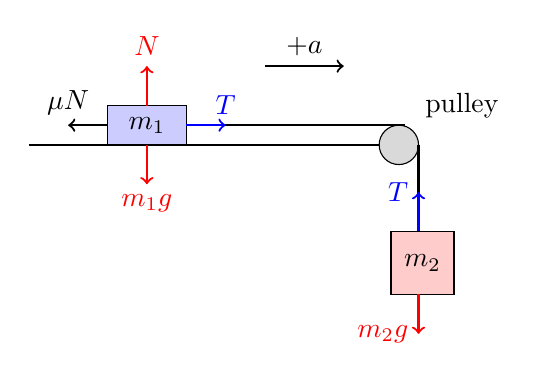
\begin{tikzpicture} 
    % Cart
    \draw[fill=blue!20] (-3, 0) rectangle (-2, 0.5) node[midway] {$m_1$};
    %\node at (-3.5, 0.25) {Cart}; % Mass label for cart
    
    % Horizontal surface for the cart
    \draw[thick] (-4, 0) -- (0.5, 0);
    
    % Pulley setup
    \draw[fill=gray!30] (0.7, 0) circle (0.25); % Horizontal pulley
    
    % String segments
    \draw[thick] (-2, 0.25) -- (0.775, 0.25); % String from cart to first pulley
    \draw[thick] (0.95, 0) -- (0.95, -1); % String from first pulley to second pulley
    
    % Hanging weight (m2)
    \node[draw, fill=red!20, minimum width=0.8cm, minimum height=0.8cm] at (1, -1.5) {$m_2$};
    
    % Force arrows on m1 (Cart)
    \draw[->, thick, red] (-2.5, 0.5) -- ++(0, 0.5) node[anchor=south] {$N$}; % Normal force
    \draw[->, thick, red] (-2.5, 0) -- ++(0, -0.5) node[anchor=north] {$m_1 g$}; % Weight of the cart
    \draw[->, thick, blue] (-2, 0.25) -- ++(0.5, 0) node[anchor=south] {$T$}; % Tension
    \draw[->, thick, black] (-3,0.25) -- ++(-0.5,0) node[anchor=south] {$\mu N$}; % friction
    
    % Force arrows on m2 (Hanging weight)
    \draw[->, thick, red] (0.95, -1.9) -- ++(0, -0.5) node[anchor=east] {$m_2 g$}; % Gravity on hanging weight
    \draw[->, thick, blue] (0.95, -1.1) -- ++(0, 0.5) node[anchor=east] {$T$}; % Tension
    
    \draw[->, thick, black] (-1, 1) -- ++(1, 0);
    \node at (-0.5, 1.25) {$+a$};
    
    % Labels for pulleys
    \node at (1.5, 0.5) {pulley};
\end{tikzpicture}
\end{center}
\caption{\label{fig:setup} Half-Atwood machine setup for testing Newton's second law, modified from \cite{canada-2024-experimental}.}
\end{figure}

For the system in \cref{fig:setup}, the equations of motion can be easily derived by writing Newton's second law for both the total cart mass ($m_1$) and the hanging mass ($m_2$) \cite{tipler, barrons}:
\begin{align}
T - m_1 g \mu &= m_1 a, \label{eq:cart}\\
m_2 g - T &= m_2 a, \label{eq:hanging}
\end{align}
where $T$ is tension in the string, $g=\qty{9.81}{\meter\per\second\squared}$ is the acceleration of gravity, and $\mu$ is a coefficient of friction associated with the cart. Combining \cref{eq:cart,eq:hanging} gives the acceleration of the system \cite{tipler,barrons}:
\begin{equation}
a = \dfrac{m_2}{m_1+m_2} g - \dfrac{m_1}{m_1+m_2} \mu g.
\label{eq:fricdimensional}
\end{equation}

Several studies have recently tested the validity of \cref{eq:n2l}, including studies conducted with constant force and varying cart mass  \cite{arenas-2024-testing,avalur-2024-verifying,canada-2024-experimental,kishore-2024-relationship,yagnyeshwaran-2024-verifying}, as well as studies in which the hanging mass provided varying external force on the system \cite{govardhanen-2024-newtons,kedharnath-2024-examining,krasnopolsky-2024-testing}. Curiously, all the studies \cite{govardhanen-2024-newtons,kedharnath-2024-examining,krasnopolsky-2024-testing} conducted with varying force ($m_2g$) also had varying total system mass ($m_1+m_2$), potentially confounding the effects of force versus mass. \cite{perle-2024-experimental} did not systematically vary $m_1$ or $m_2$ and was limited in conclusions regarding \cref{eq:n2l}; while \cite{barone-2024-investigating} had no means to measure accceleration. \cite{krasnopolsky-2024-testing} exceeded the acceleration of gravity $g$ in observed results, while \cite{govardhanen-2024-newtons} observed extremely low values of system acceleration, possibly due to incorrectly recorded mass $m_1$. Many studies also suffered from having only minimal replicates of measured data. All \cite{arenas-2024-testing,avalur-2024-verifying,canada-2024-experimental,kishore-2024-relationship,yagnyeshwaran-2024-verifying,govardhanen-2024-newtons,kedharnath-2024-examining,krasnopolsky-2024-testing,perle-2024-experimental} claimed to be affected by friction; some also noted timing inaccuracies, factors related to the clean release of the system from rest, and various other ``human error[s]'' as sources of experimental error. 

Here, we wish to combine the results of \cite{arenas-2024-testing,avalur-2024-verifying,canada-2024-experimental,kishore-2024-relationship,yagnyeshwaran-2024-verifying,govardhanen-2024-newtons,kedharnath-2024-examining,krasnopolsky-2024-testing,perle-2024-experimental}. The combined dataset could potentially overcome many of the shortfalls of each individual study, including items like release, timing inaccuracies, and ``human error'' since these are presumably randomized out among the different workers. With a larger dataset it may also be possible to test the claim the friction affected the results.  Since some previous studies \cite{arenas-2024-testing,avalur-2024-verifying,canada-2024-experimental,kishore-2024-relationship,yagnyeshwaran-2024-verifying} were done with constant force, while others were done with varying hanging mass \cite{govardhanen-2024-newtons,kedharnath-2024-examining,krasnopolsky-2024-testing}, we nondimensionalize \cref{eq:fricdimensional}, to combine the various datasets into a single coherent picture and collapse four independent variables ($m_1$, $m_2$, $g$, and $\mu$) into two ($\hat{m}$, $\mu$). 

Defining nondimensional system acceleration $\hat{a} = \dfrac{a}{g}$ and nondimensional hanging mass $\hat{m} = \dfrac{m_2}{m_1+m_2}$ gives
\begin{equation}
\hat{a} = \hat{m} - (1-\hat{m}) \mu,
\end{equation}
\begin{equation}
\hat{a} = (1+\mu) \hat{m} - \mu,
\end{equation}
\begin{equation}
\hat{a} = 
\begin{cases}
(1+\mu) \hat{m} - \mu & \hat{m} \geq \dfrac{\mu}{1+\mu}, \\
0 & \hat{m} < \dfrac{\mu}{1+\mu}.
\end{cases}
\label{eq:fricdimensionless}
\end{equation}
The condition $\hat{m}=\dfrac{\mu}{1+\mu}$ is equivalent to $m_2=\mu m_1$; below this critical value static friction will keep the system from moving. 

For the case of no friction, \cref{eq:fricdimensional} reduces to
\begin{equation}
a = \dfrac{m_2}{m_1+m_2} g,
\label{eq:nofricdimensional}
\end{equation}
while \cref{eq:fricdimensionless} becomes
\begin{equation}
\hat{a} = \hat{m}.
\label{eq:nofricdimensionless}
\end{equation}

\Cref{fig:prediction} shows predictions for $\hat{a}$ based on whether friction is significant \cref{eq:fricdimensionless} or not \cref{eq:nofricdimensionless}. If the measured data fail to follow either of these relationships, then the models from \cref{eq:fricdimensional} are wrong, indicating either missing or unmodeled forces, or that \cref{eq:n2l} is invalid in this system. 
\begin{figure}
\begin{center}
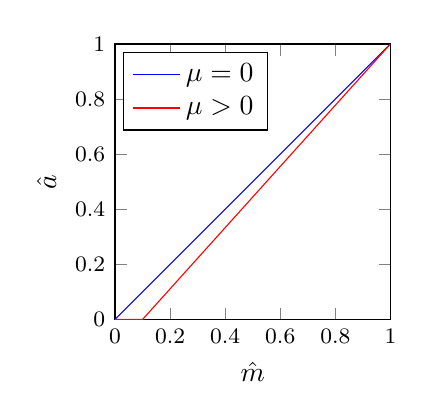
\begin{tikzpicture}
\begin{axis}[
%title={Mass on String vs. Weight (Tension)},
xlabel={$\hat{m}$},
ylabel={$\hat{a}$},
xmin=0, xmax=1.0, 
ymin=0, ymax=1.0,
%xtick={0,0.500,1.000,1.500,2.000},
%ytick={0,5,10,15,20,25},
%grid=both,
legend pos=north west,
every axis label/.style={font=\normalsize},
every tick label/.style={font=\footnotesize},
width=2in,
height=2in,
]
\addplot[color=blue] coordinates {
(0.0, 0.0)
(1.0, 1.0)
};
\addlegendentry{$\mu=0$}
\addplot[color=red] coordinates {
(0.0, 0.0)
(0.1, 0.0)
(1.0, 1.0)
};
\addlegendentry{$\mu>0$}
%\addlegendentry{Measured Data}
\end{axis}
\end{tikzpicture}
\end{center}
\caption{\label{fig:prediction} Predicted relationships between $\hat{m}$ and $\hat{a}$ for case with friction, \cref{eq:fricdimensionless} (red)  and frictionless case, \cref{eq:nofricdimensionless} (blue).}
\end{figure}






\section{Methods and materials}
Data from \cite{arenas-2024-testing,avalur-2024-verifying,canada-2024-experimental,kishore-2024-relationship,yagnyeshwaran-2024-verifying,govardhanen-2024-newtons,kedharnath-2024-examining,krasnopolsky-2024-testing,perle-2024-experimental} for $m_1$, $m_2$, and $a_{meas}$ were combined for analysis and plotting in R \cite{R-2024} using the \texttt{ggplot2} library \cite{ggplot2-2024}. The original data from \cite{arenas-2024-testing,avalur-2024-verifying,canada-2024-experimental,kishore-2024-relationship,yagnyeshwaran-2024-verifying,govardhanen-2024-newtons,kedharnath-2024-examining,krasnopolsky-2024-testing,perle-2024-experimental} were collected using half-Atwood machine setups (PASCO Scientific; Roseville, CA); accelerations $a_{meas}$ were estimated by timing the time $t_{meas}$ for the system to move a distance $d$ from rest. For data from \cite{govardhanen-2024-newtons}, $m_1$ was corrected to be \qty{2.5}{\kilo\gram}. Data from \cite{krasnopolsky-2024-testing} at highest two values of $m_2$ show timing issues with very short times, resulting in non-physical estimates that exceed the acceleration of gravity; these were removed from analysis.

The mass was nondimensionalized using
\begin{equation}
\hat{m} = \dfrac{m_2}{m_1+m_2}, \label{eq:mhat}
\end{equation}
while the measured system acceleration was nondimensionalized using
\begin{equation}
\hat{a} = \dfrac{a}{g}. \label{eq:ahat}
\end{equation}
These were plotted in R using the \texttt{ggplot2} library; further statistical analyses were carried out using a linear model (\texttt{lm}) \cite{R-2024,ggplot2-2024}. Data and code are available at \url{https://github.com/devangel77b/426ahacker-lab2.1}. 





\section{Results}
\Cref{fig:results} shows the datasets from \cite{arenas-2024-testing,avalur-2024-verifying,canada-2024-experimental,kishore-2024-relationship,yagnyeshwaran-2024-verifying,govardhanen-2024-newtons,kedharnath-2024-examining,krasnopolsky-2024-testing,perle-2024-experimental} in nondimensional form \cref{eq:mhat,eq:ahat}. For these data, the best fit line is $\hat{a}=0.98\hat{m}$ (linear regression, $R^2=0.9777$, $df=95$, $p<\num{2e-16}$). The slope is not significantly different from 1.0 ($t$-test, $p=0.227$).
\begin{figure*}
\includesvg{fig2.svg}
\caption{\label{fig:results} Datasets from \cite{arenas-2024-testing,avalur-2024-verifying,canada-2024-experimental,kishore-2024-relationship,yagnyeshwaran-2024-verifying,govardhanen-2024-newtons,kedharnath-2024-examining,krasnopolsky-2024-testing,perle-2024-experimental} in nondimensional form, $\hat{a}=\dfrac{a}{g}$ and $\hat{m}=\dfrac{m_2}{m_1+m_2}$. Best fit line is $\hat{a}=0.98\hat{m}$ (linear regression, $R^2=0.9777$, $df=95$, $p<\num{2e-16}$), slope is not significantly different from 1.0 ($t$-test, $p=0.227$), providing support for \cref{eq:nofricdimensional,eq:nofricdimensionless,eq:n2l}. Data from \cite{govardhanen-2024-newtons} uses corrected value of $m_1=\qty{2.5}{\kilo\gram}$. Data from \cite{krasnopolsky-2024-testing} at highest two values of $m_2$ (top, right) show timing issues with very short times and results that exceed the acceleration of gravity and so are removed from analysis. Gray box shows area where analysis is valid.}
\end{figure*}

%\begin{figure*}
%\includesvg{fig3.svg}
%\caption{Blah. }
%\end{figure*}





\section{Discussion}
As shown in \cref{fig:results}, the combined results of \cite{arenas-2024-testing,avalur-2024-verifying,canada-2024-experimental,kishore-2024-relationship,yagnyeshwaran-2024-verifying,govardhanen-2024-newtons,kedharnath-2024-examining,krasnopolsky-2024-testing,perle-2024-experimental} are most consistent with \cref{eq:nofricdimensional,eq:nofricdimensionless}. The slope is not significantly different from one, and the intercept is not significantly different from zero; these do not support the models with friction from \cref{eq:fricdimensional,eq:fricdimensionless}. Friction does not appear to be the dominant source of experimental error, contrary to what was claimed in \cite{arenas-2024-testing,avalur-2024-verifying,canada-2024-experimental,kishore-2024-relationship,yagnyeshwaran-2024-verifying,govardhanen-2024-newtons,kedharnath-2024-examining,krasnopolsky-2024-testing,perle-2024-experimental}.

The results are consistent with Newton's second law. The models of \cref{eq:nofricdimensional,eq:nofricdimensionless} were derived from analysis of the free body diagrams in \cref{fig:setup} using \cref{eq:n2l}; good agreement of \cref{fig:results} with the predictions of \cref{eq:nofricdimensionless} supports the findings of \cite{arenas-2024-testing,avalur-2024-verifying,canada-2024-experimental,kishore-2024-relationship,yagnyeshwaran-2024-verifying,govardhanen-2024-newtons,kedharnath-2024-examining,krasnopolsky-2024-testing,perle-2024-experimental} and the validity of Newton's second law in this system. 

The largest and most notable experimental error appears to be at high values of $m_2$ in data from \cite{krasnopolsky-2024-testing}. It is possible that the highest values of $m_2$ and $a$ becomes prone to timing errors during data gathering. Most of the measured data from \cite{arenas-2024-testing,avalur-2024-verifying,canada-2024-experimental,kishore-2024-relationship,yagnyeshwaran-2024-verifying,govardhanen-2024-newtons,kedharnath-2024-examining,krasnopolsky-2024-testing,perle-2024-experimental} are for $\hat{m}<0.3$; while data above this range comes mainly from one study \cite{krasnopolsky-2024-testing}. Future measurements with this system should focus on filling in gaps in the region $0.3<\hat{m}<1$.  

\section{Acknowledgements}
APH and LR devised the analyses and wrote the manuscript. 

\bibliography{hacker.bib}
\end{document}
